\documentclass{article} % For LaTeX2e
\usepackage{nips13submit_e,times}
\usepackage{hyperref}
\usepackage{float}
\usepackage{url}
\usepackage[pdftex]{graphicx} 
\usepackage{lipsum}
\usepackage{listings}
\usepackage{geometry}
\usepackage{hyperref}
\usepackage{booktabs}
%\documentstyle[nips13submit_09,times,art10]{article} % For LaTeX 2.09
%\geometry{verbose,tmargin=1in,bmargin=1in,lmargin=1in,rmargin=1in, left=1.5cm, right=1.3cm}

\title{Exploratory Analysis of the Crime Reporting Pattern in Oakland using MySQL and Jupyter Notebook}



\author{
	Jiarong Ye\\
	College of Engineering\\
	\texttt{jxy225@psu.edu} \\
	\And
	Yichi Qian\\
	College of Engineering\\
	\texttt{yzq5048@psu.edu} \\
	\\
	\And
	Han Shao\\
	College of IST \\
	\texttt{hbs5203@psu.edu} \\	
}






\newcommand{\fix}{\marginpar{FIX}}
\newcommand{\new}{\marginpar{NEW}}

\nipsfinalcopy 

\begin{document}


\maketitle

\begin{abstract}

[Please complete this part ...]

\end{abstract}

\section{Introduction}

[Please complete this part ...]

\section{Data Set}


The crime statistics dataset in Oakland from 2011 to 2016 is collected from Kaggle \cite{kaggle}. It is published and maintained by the city of Oakland. 
The attributes contained in the dataset include:
\begin{itemize}
\item  Agency
\item  Create Time
\item  Location
\item  Area Id
\item  Beat
\item  Priority
\item  Incident Type Id
\item  Incident Type Description
\item  Event Number
\item  Closed Time
\item  \textbf{Average Resolving Time} (\textit{calculated by subtracting \textbf{Create Time} from \textbf{Closed Time}})

\end{itemize}


\section{MySQL Data Loading Pipeline}


Why choose MySQL: [please complete this part ...]

\textit{it would be better if you can do a comparison between MySQL and other databases, list the pros and cons and illustrate why MySQL should be chosen}


Regarding the advantages and drawbacks of several databases discussed, the database we choose for the class project is MySQL (local server). And in order to implement the cleaning and visualization of the aggregated data extracted from databases afterwards, we wrote a data processing pipeline to combine the merits of Jupyter Notebook and MySQL and present our observation with proper interpretability through tables and graphs. The python package we applied to connect to the MySQL local server is PyMySQL \cite{pymysql}, by which we were able to integrate the database and the programming environment together.


Then we construct a \hyperref[appendix:preprocess]{pipeline} to:

\begin{itemize}
	\item clean the \textbf{location} attribute of the raw dataset since its format is not consistent in all the 6 tables (from 2011 to 2016);
	\item format the \textbf{Create/Closed Time} attribute raw dataset to be MySQL compatible;
	\item create tables in MySQL
	\item insert cleaned data into MySQL
	\item extract data from MySQL given a query
\end{itemize} 

\section{Exploratory Data Analysis \textit{}}

\subsection{What crime has the highest occurrence all across Oakland?}

\begin{figure}[H]
	\begin{center}
		%\framebox[4.0in]{$\;$}
		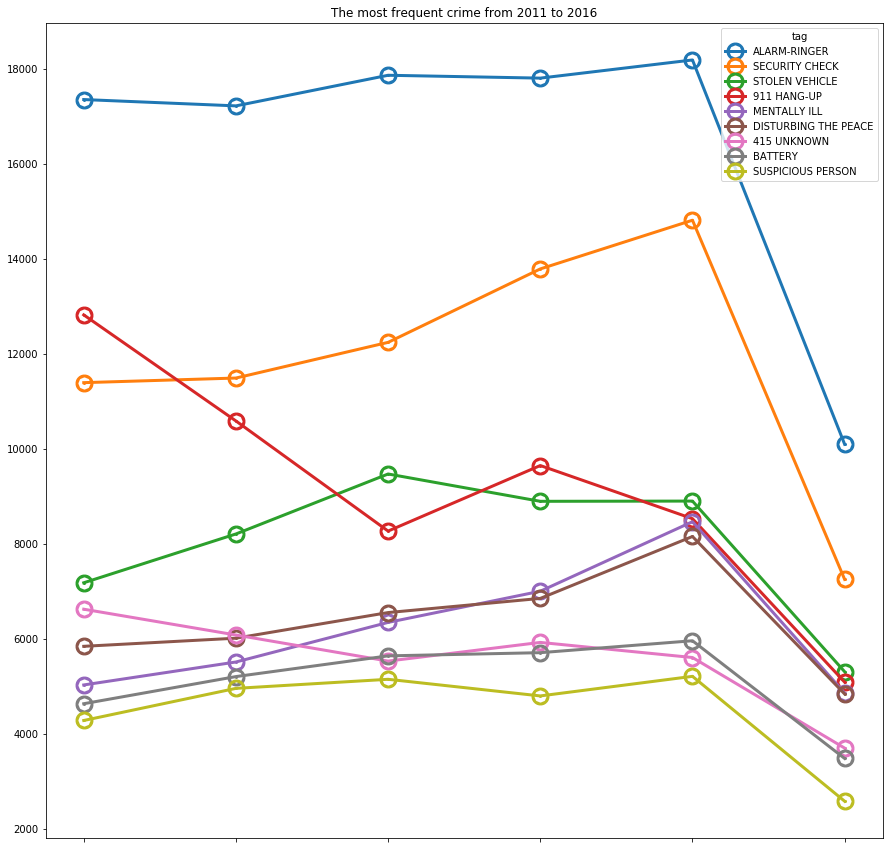
\includegraphics[height=8cm, width=11cm]{1.png}
	\end{center}
	\caption{\hyperref[appendix:plot1]{The most frequent crime in Oakland from 2011 to 2016}}
\end{figure}


\subsection{What crime has the highest occurrence in each location?}


\begin{figure}[H]
	\begin{center}
		%\framebox[4.0in]{$\;$}
		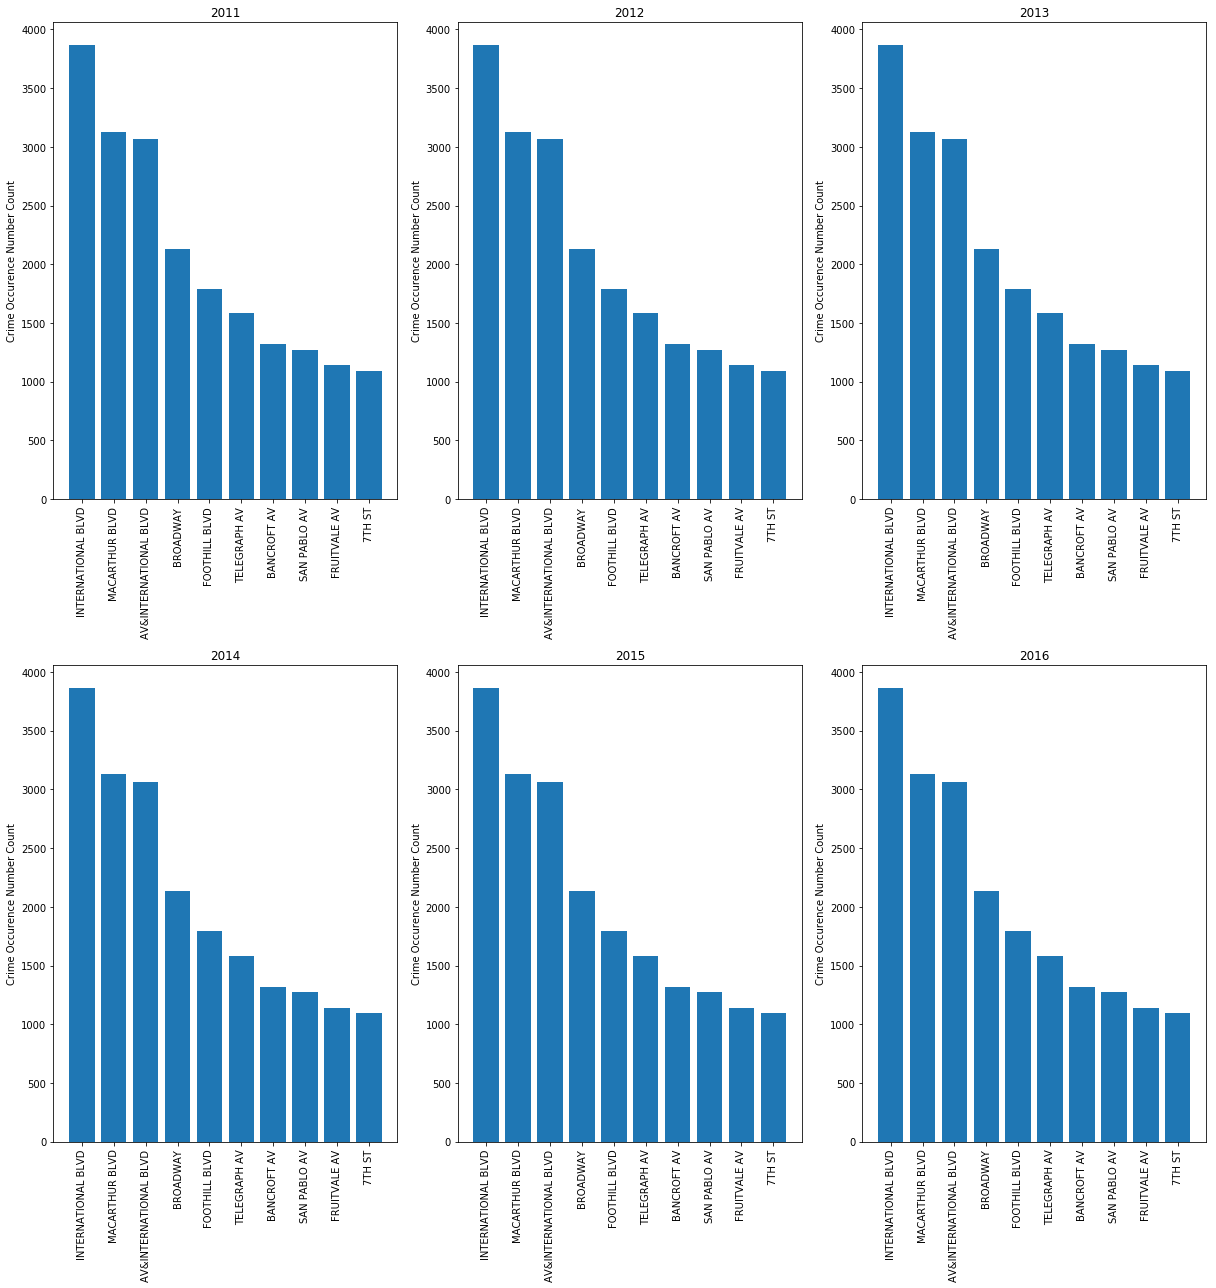
\includegraphics[height=10cm, width=15cm]{2.png}
	\end{center}
	\caption{\hyperref[appendix:plot1]{Locations with the most frequent crime in Oakland from 2011 to 2016}}
\end{figure}

The top locations with the most crime reporting counts across 6 years:

\begin{center}
\begin{tabular}{|l|p{3cm}|p{2.2cm}|r|r|r|r|}
	\toprule
	Year & INTERNATIONAL BLVD &  MACARTHUR BLVD &  BROADWAY &  FOOTHILL BLVD &  TELEGRAPH AV &  7TH ST \\
	\midrule
	2011 &                3866 &            3129 &      2132 &           1791 &          1584 &    1093 \\
	2012 &                3658 &            3335 &      2167 &           1649 &          1623 &    1183 \\
	2013 &                3647 &            3002 &      2036 &           1650 &          1558 &    1246 \\
	2014 &                3713 &            2812 &      1996 &           1774 &          1573 &    1285 \\
	2015 &                3695 &            3105 &      2407 &           1753 &          1507 &    1569 \\
	2016 &                2156 &            1813 &      1476 &           1052 &           875 &    1224 \\
	\bottomrule
\end{tabular}
\end{center}

\begin{figure}[H]
	\begin{center}
		%\framebox[4.0in]{$\;$}
		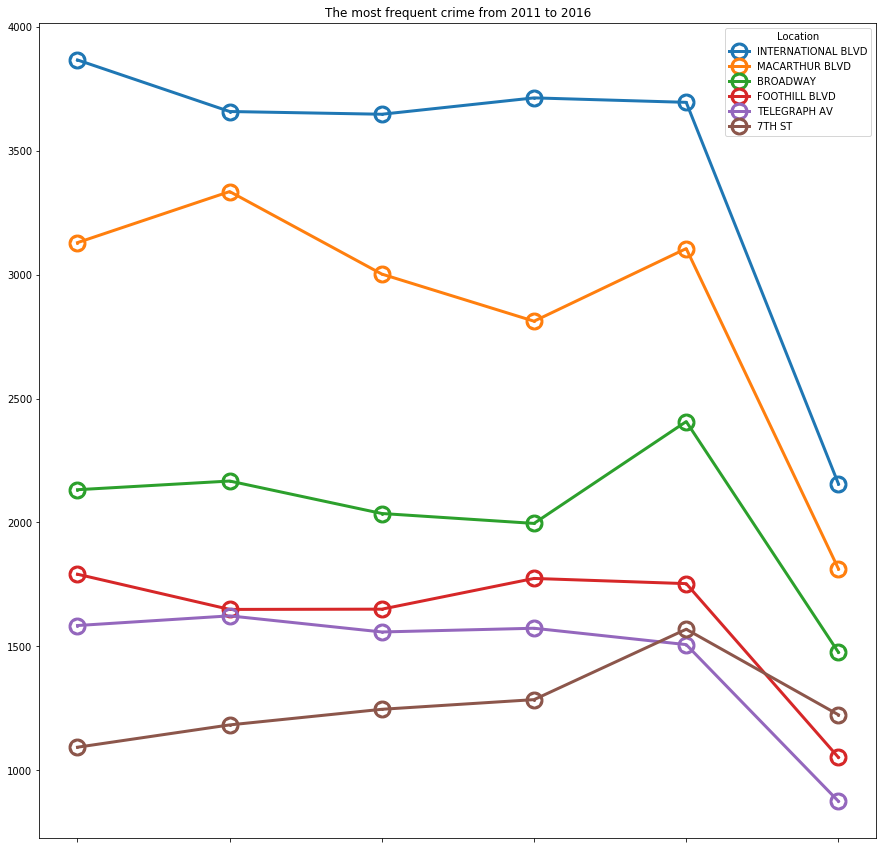
\includegraphics[height=8cm, width=11cm]{3.png}
	\end{center}
	\caption{\hyperref[appendix:plot2]{The location with highest crime rate from 2011 to 2016}}
\end{figure}

Therefore, observing from the graph above, the \textbf{International Blvd} is the place with the highest crime reporting rate.


\subsubsection{What crime has the highest occurrence in International Blvd?}

The top incident types with the highest reporting counts in \textbf{International Blvd} across 6 years:

\begin{center}
\begin{tabular}{|p{1cm}|p{6cm}|p{3cm}|}
	\toprule
	{} &            crime type &  occurrence \\
	\midrule
	0 &          ALARM-RINGER &        1979 \\
	1 &           911 HANG-UP &        1646 \\
	2 &  DISTURBING THE PEACE &        1009 \\
	3 &          MENTALLY ILL &         911 \\
	4 &           415 UNKNOWN &         984 \\
	5 &               BATTERY &         723 \\
	6 &        SECURITY CHECK &        1456 \\
	7 &        STOLEN VEHICLE &         725 \\
	\bottomrule
\end{tabular}
\end{center}


\begin{figure}[H]
	\begin{center}
		%\framebox[4.0in]{$\;$}
		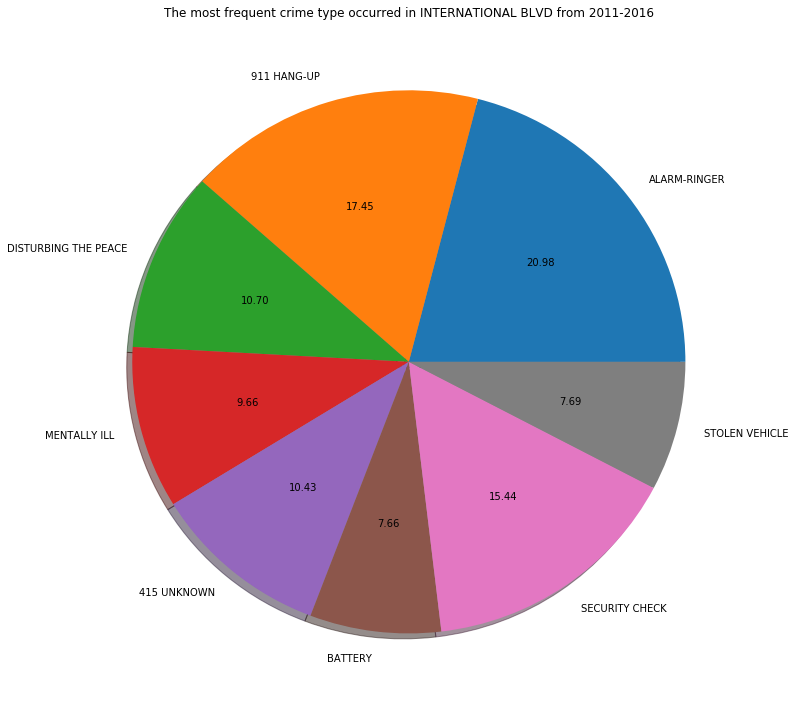
\includegraphics[height=8cm, width=8cm]{4.png}
	\end{center}
	\caption{\hyperref[appendix:plot3]{The most frequent crime type reported in International Blvd from 2011-2016}}
\end{figure}




\subsection{What is the incident solving time for each incident?}


\begin{figure}[H]
	\begin{center}
		%\framebox[4.0in]{$\;$}
		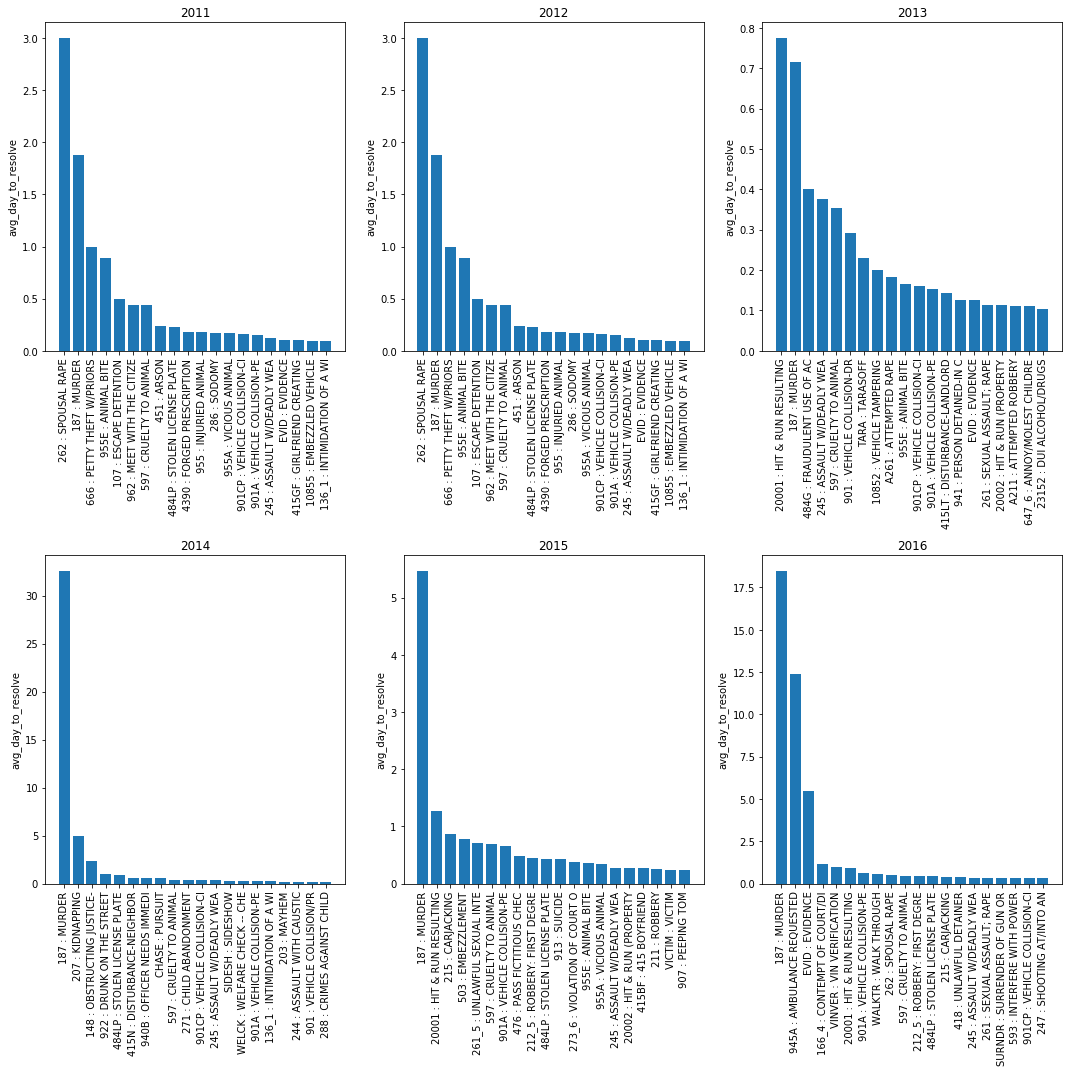
\includegraphics[height=8cm, width=15cm]{5.png}
	\end{center}
	\caption{\hyperref[appendix:plot4]{The average resolving time of crime types in Oakland from 2011-2016}}
\end{figure}


The average resolving days of the top incident types that took the longest days to resolve from 2011 to 2016:

\begin{center}
\begin{tabular}{|l|r|r|r|r|r|}
	\toprule
	 &   MURDER &  ANIMAL BITE &  CRUELTY TO ANIMAL &  VICIOUS ANIMAL &  VEHICLE COLLISION-PE \\
	\midrule
	2011 &   1.8750 &       0.8884 &             0.4347 &          0.1660 &                0.1542 \\
	2012 &   0.7143 &       0.1660 &             0.3531 &          0.0738 &                0.1524 \\
	2013 &  32.5758 &       0.1453 &             0.4140 &          0.1200 &                0.2821 \\
	2014 &   5.4688 &       0.3646 &             0.6883 &          0.3364 &                0.6486 \\
	2015 &  18.4839 &       0.1588 &             0.4433 &          0.1555 &                0.6310 \\
	2016 &   5.4118 &       0.2806 &             0.5074 &          0.1727 &                0.1474 \\
	\bottomrule
\end{tabular}
\end{center}

\begin{figure}[H]
	\begin{center}
		%\framebox[4.0in]{$\;$}
		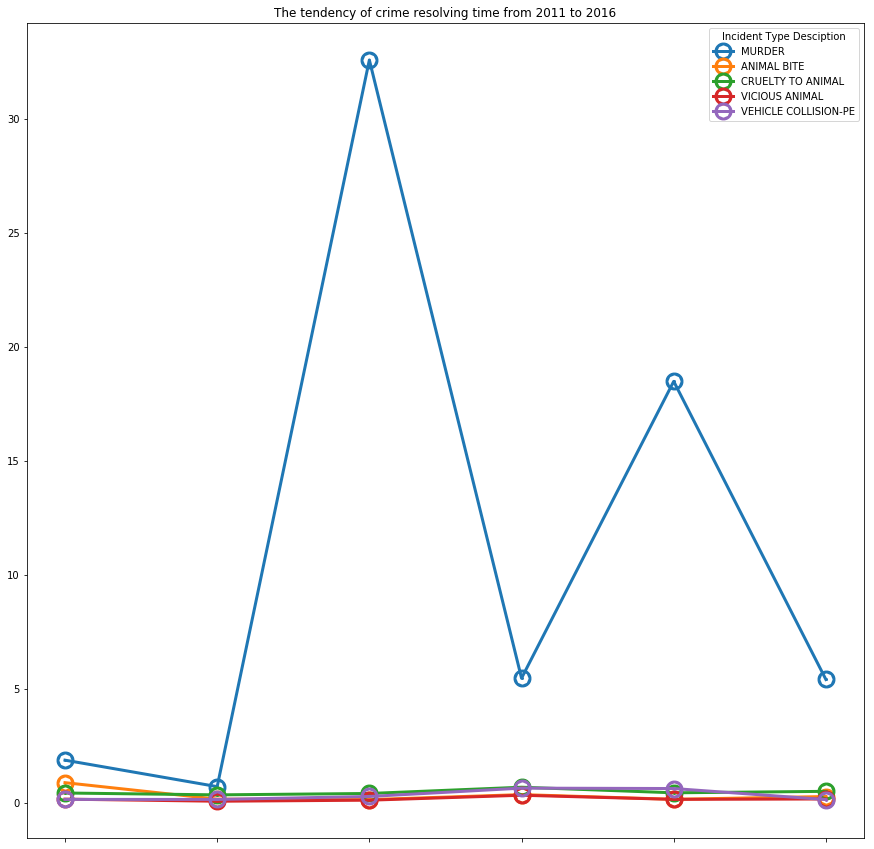
\includegraphics[height=8cm, width=10cm]{6.png}
	\end{center}
	\caption{\hyperref[appendix:plot4]{The time cost trend of top incident types that took the longest resolving time  from 2011 to 2016}}
\end{figure}



\section{Conclusion}


[Please complete this part ...]

\[\]


\bibliographystyle{plain}
\bibliography{ref}

\section{Appendix: Python Code}

\[\]

\appendix

\lstset{language=python}
\lstset{frame=lines}
\lstset{caption={Import Packages}}
\lstset{basicstyle=\footnotesize}
\begin{lstlisting}
import pandas as pd
import os
import re
import numpy as np
import pymysql 
from datetime import datetime
import matplotlib.pyplot as plt
import seaborn as sns
\end{lstlisting}



\label{appendix:preprocess}
\lstset{language=python}
\lstset{frame=lines}
\lstset{caption={Clean address for data in 2012 and 2014}}
\lstset{basicstyle=\footnotesize}
\begin{lstlisting}
PATH = 'oakland-crime-statistics-2011-to-2016/'
FILE_2011 = PATH+'records-for-2011.csv'
FILE_2012 = PATH+'records-for-2012.csv'
FILE_2013 = PATH+'records-for-2013.csv'
FILE_2014 = PATH+'records-for-2014.csv'
FILE_2015 = PATH+'records-for-2015.csv'
FILE_2016 = PATH+'records-for-2016.csv'

def convert_location_col(df, filename):
	reg_pattern = '\"address\":\"([A-Za-z0-9\s./#\(\),-]+)\"'
	address_lst = list(map(lambda x: re.findall(pattern=reg_pattern,
		 string=df['Location 1'][x].replace('&amp;', ' ')), range(len(df))))
	address_lst_flattened = []
	for i in range(len(address_lst)):
		try:
			address_lst_flattened.append(address_lst[i][0])
		except Exception as e:
			address_lst_flattened.append(np.nan)
	df['Location'] = address_lst_flattened
	df = df.drop(columns=['Location 1'])
	df = pd.concat([df.iloc[:,:2], df.Location, df.iloc[:,2:-1]], axis=1)
	df.to_csv(filename, index=None)
	return df

df1 = convert_location_col(pd.read_csv(FILE_2012), FILE_2012)
df2 = convert_location_col(pd.read_csv(FILE_2014), FILE_2014)
\end{lstlisting}


\lstset{language=python}
\lstset{frame=lines}
\lstset{caption={Convert time format to be MySQL compatible}}
\lstset{basicstyle=\footnotesize}
\begin{lstlisting}
def convert_time_sql_format():
    columns = ['Create Time', 'Closed Time']
    for y in range(1,7):
    	filename = PATH + 'records-for-201{}.csv'.format(y)
    	df = pd.read_csv(filename)
    	for column in columns:
    		tmp = []
    		df = df.iloc[df[column].dropna().index, :].reset_index(drop=True)
    		for i in df[column]:
    			ymy = i.split('T')[0]
    			hms = i.split('T')[1]
    			splited_lst = ymy.split('-')
    			year = splited_lst[0]
    			month = splited_lst[1][1:] if splited_lst[1].startswith('0')
    							 else splited_lst[1]
    			day = splited_lst[2][1:] if splited_lst[2].startswith('0')
    							else splited_lst[2]
    			splited_lst = hms.split(':')
    			hour = splited_lst[0][1:] if splited_lst[0].startswith('0')
    							else splited_lst[0]
    			minute = splited_lst[1][1:] if splited_lst[1].startswith('0')
    							else splited_lst[1]
    			second = splited_lst[2][1:] if splited_lst[2].startswith('0')
    							else splited_lst[2]
    			tmp.append(datetime(int(year), int(month), int(day),
    						int(hour), int(minute), int(second)))
    		df[column] = pd.DataFrame(tmp)
	df['Days to Resolve'] = pd.DataFrame(list(map(lambda x: x.days,
						 df[columns[1]] - df[columns[0]])))
	df['Area Id'] = df['Area Id'].fillna(value=0)
	df['Priority'] = df['Priority'].dropna(axis=0)
	df['Incident Type Id'] = df['Incident Type Id'].dropna(axis=0)
	df['Event Number'] = df['Event Number'].dropna(axis=0)
	df.to_csv(filename, index=None)
	
convert_time_sql_format()
\end{lstlisting}


\lstset{language=python}
\lstset{frame=lines}
\lstset{caption={Load data into MySQL}}
\lstset{basicstyle=\footnotesize}
\begin{lstlisting}
class DataSqlLoader:
   def __init__(self, database):
      # connect to mysql local server
      self.database = database
      self.db = pymysql.Connect(
      	host = 'localhost',	
      	user = 'root',	
      	passwd = '',
      	db=self.database)
      self.c = self.db.cursor()

   def creat_tables(self):
      for year in range(1, 7):
         try:
            self.c.execute('''
			CREATE TABLE IF NOT EXISTS crimedata_201{}
			(
			`Agency`                   VARCHAR(5)   NULL,
			`Create Time`              DATETIME     NULL,
			Location                   VARCHAR(100) NULL,
			`Area Id`                  VARCHAR(5)   NULL,
			Beat                       VARCHAR(10)  NULL,
			Priority                   Double       NULL,
			`Incident Type Id`         VARCHAR(10)  NULL,
			`Incident Type Description` TEXT         NULL,
			`Event Number`             VARCHAR(30)  NOT NULL
			PRIMARY KEY,
			`Closed Time`              DATETIME     NULL,
			`Days to Resolve`          INT          NULL,
			CONSTRAINT crimedata_2011_EventNumber_uindex
			UNIQUE (`Event Number`)
			);
			'''.format(year))
           except Exception as e:
               print(e) 
   
   def insert_into_tables(self, filename, tablename):
      query = '''
         LOAD DATA INFILE '{}'
         INTO TABLE {} fields terminated by ',' lines terminated by '\r\n'
         '''.format(filename, tablename)
      try:
        self.c.execute(query)
      except Exception as e:
        print(e)
          
   def drop_table(self, tablename):
     try:
       self.c.execute('''drop table {}'''.format(tablename))
     except Exception as e:
       print(e)


   def get_sample(self, table, limit=None):
     if limit == None:
       query = '''SELECT * FROM {};'''.format(table)
     else:
       query = '''SELECT * FROM {} limit {};'''.format(table, limit)
       pd.read_sql(sql=query, con=self.db)
     return pd.read_sql(sql=query, con=self.db)

   def sql_query(self, query):
     try:
       return pd.read_sql(sql=query, con=self.db)
     except Exception as e:
       print(e)

  def close(self):
     self.db.close()
     
dsl = DataSqlLoader('ds220')
dsl.creat_tables()
dsl.insert_into_tables(FILE_2011, 'crime_2011')
dsl.insert_into_tables(FILE_2012, 'crime_2012')
dsl.insert_into_tables(FILE_2013, 'crime_2013')
dsl.insert_into_tables(FILE_2014, 'crime_2014')
dsl.insert_into_tables(FILE_2015, 'crime_2015')
dsl.insert_into_tables(FILE_2016, 'crime_2016')
\end{lstlisting}


\label{appendix:plot1}
\lstset{language=python}
\lstset{frame=lines}
\lstset{showstringspaces=false}
\lstset{caption={What crime has the highest occurrence all across Oakland}}
\lstset{basicstyle=\footnotesize}
\begin{lstlisting}
query = '''
select t1.tag, t1.cnt, t2.cnt, t3.cnt, t4.cnt, t5.cnt, t6.cnt
	from
		(select `Incident Type Desciption` as tag, count(*) as cnt
		from crimedata_2011
		group by `Incident Type Desciption`
		order by cnt desc
		limit 10) as t1
	inner join
		(select `Incident Type Desciption` as tag, count(*) as cnt
		from crimedata_2012
		group by `Incident Type Desciption`
		order by cnt desc
		limit 10) as t2
	inner join 
		(select `Incident Type Desciption` as tag, count(*) as cnt
		from crimedata_2013
		group by `Incident Type Desciption`
		order by cnt desc
		limit 10) as t3
	inner join 
		(select `Incident Type Desciption` as tag, count(*) as cnt
		from crimedata_2014
		group by `Incident Type Desciption`
		order by cnt desc
		limit 10) as t4
	inner join 
		(select `Incident Type Desciption` as tag, count(*) as cnt
		from crimedata_2015
		group by `Incident Type Desciption`
		order by cnt desc
		limit 10) as t5
	inner join 
		(select `Incident Type Desciption` as tag, count(*) as cnt
		from crimedata_2016
		group by `Incident Type Desciption`
		order by cnt desc
		limit 10) as t6
	on t1.tag=t2.tag
	and t2.tag=t3.tag
	and t3.tag=t4.tag
	and t4.tag=t5.tag
	and t5.tag=t6.tag;
	'''
highest_freq_crime_all_6_years = dsl.sql_query(query=query)
highest_freq_crime_all_6_years = highest_freq_crime_all_6_years.set_index('tag').transpose()
highest_freq_crime_all_6_years.plot(legend=True, figsize=(15,15), 
		marker='.', lw=3, mew=15, title='The most frequent crime from 2011 to 2016')
\end{lstlisting}

\label{appendix:plot2}
\lstset{language=python}
\lstset{frame=lines}
\lstset{caption={What crime has the highest occurrence in each location?}}
\lstset{basicstyle=\footnotesize}
\begin{lstlisting}
# each year
plt.figure(figsize=(17, 18))
for year in range(1, 7):
	location_cnt = dsl.sql_query("""select Location,
	`Incident Type Desciption`,
	count(*) cnt
	from crimedata_2011
	group by Location
	order by cnt desc
	limit 10;
	""".format(year))
	print('The top 3 location with highest crime rate in year 201{}:'.format(year))
	print(incident_location_cnt.iloc[:3, :].values)
	print('\n')
	
	plt.subplot(2, 3, year)
	plt.bar(x=location_cnt.Location, height=location_cnt.cnt)
	plt.xticks(rotation=90)
	plt.ylabel('Crime Occurence Number Count')
	plt.title('201{}'.format(year))
	plt.tight_layout()
plt.show()

# trend across 6 years
query = '''
	select t1.Location, 
		t1.cnt as count_2011, 
		t2.cnt as count_2012, 
		t3.cnt as count_2013, 
		t4.cnt as count_2014, 
		t5.cnt as count_2015, 
		t6.cnt as count_2016
	from
		(select Location,
		count(*) cnt
		from crimedata_2011
		group by Location
		order by cnt desc limit 10) as t1
	inner join
		(select Location,
		count(*) cnt
		from crimedata_2012
		group by Location
		order by cnt desc limit 10) as t2
	inner join 
		(select Location,
		count(*) cnt
		from crimedata_2013
		group by Location
		order by cnt desc limit 10) as t3
	inner join 
		(select Location,
		count(*) cnt
		from crimedata_2014
		group by Location
		order by cnt desc limit 10) as t4
	inner join 
		(select Location,
		count(*) cnt
		from crimedata_2015
		group by Location
		order by cnt desc limit 10) as t5
	inner join 
		(select Location,
		count(*) cnt
		from crimedata_2016
		group by Location
		order by cnt desc limit 10) as t6
	on t1.Location=t2.Location
	and t2.Location=t3.Location
	and t3.Location=t4.Location
	and t4.Location=t5.Location
	and t5.Location=t6.Location;
	'''
highest_freq_crime_location_all_6_years = dsl.sql_query(query=query)
highest_freq_crime_location_all_6_years = highest_freq_crime_location_all_6_years
							.set_index('Location').transpose()
highest_freq_crime_location_all_6_years.plot(legend=True, figsize=(15,15), 
			marker='.', lw=3, mew=15, 
			title='The location with highest crime rate from 2011 to 2016')
\end{lstlisting}

\label{appendix:plot3}
\lstset{language=python}
\lstset{frame=lines}
\lstset{caption={What crime has the highest occurrence in International Blvd?}}
\lstset{basicstyle=\footnotesize}
\begin{lstlisting}
query = '''
	select t1.tag, 
			t1.cnt, 
			t2.cnt, 
			t3.cnt, 
			t4.cnt, 
			t5.cnt, 
			t6.cnt
	from
		(select `Incident Type Desciption` as tag, count(*) as cnt
		from crimedata_2011
		where Location='INTERNATIONAL BLVD'
		group by `Incident Type Desciption`
		order by cnt desc
		limit 10) as t1
	inner join
		(select `Incident Type Desciption` as tag, count(*) as cnt
		from crimedata_2012
		where Location='INTERNATIONAL BLVD'
		group by `Incident Type Desciption`
		order by cnt desc
		limit 10) as t2
	inner join 
		(select `Incident Type Desciption` as tag, count(*) as cnt
		from crimedata_2013
		where Location='INTERNATIONAL BLVD'
		group by `Incident Type Desciption`
		order by cnt desc
		limit 10) as t3
	inner join 
		(select `Incident Type Desciption` as tag, count(*) as cnt
		from crimedata_2014
		where Location='INTERNATIONAL BLVD'
		group by `Incident Type Desciption`
		order by cnt desc
		limit 10) as t4
	inner join 
		(select `Incident Type Desciption` as tag, count(*) as cnt
		from crimedata_2015
		where Location='INTERNATIONAL BLVD'
		group by `Incident Type Desciption`
		order by cnt desc
		limit 10) as t5
	inner join 
		(select `Incident Type Desciption` as tag, count(*) as cnt
		from crimedata_2016
		where Location='INTERNATIONAL BLVD'
		group by `Incident Type Desciption`
		order by cnt desc
		limit 10) as t6
	on t1.tag=t2.tag
	and t2.tag=t3.tag
	and t3.tag=t4.tag
	and t4.tag=t5.tag
	and t5.tag=t6.tag;
	'''
highest_freq_crime_internationalblvd_all_6_years = dsl.sql_query(query=query)
highest_freq_crime_internationalblvd_all_6_years =
	 pd.concat([highest_freq_crime_internationalblvd_all_6_years.tag, 
		highest_freq_crime_internationalblvd_all_6_years.sum(axis=1)], axis=1)
highest_freq_crime_internationalblvd_all_6_years.columns = ['crime type', 'occurrence']

# high frequency crime type in the location with the highest crime rate

plt.figure(figsize=(10, 10))
plt.pie(highest_freq_crime_internationalblvd_all_6_years.occurrence,
	labels=highest_freq_crime_internationalblvd_all_6_years['crime type'],
	autopct = '%.2f',
	shadow=True)
plt.title('The most frequent crime type occurred in INTERNATIONAL BLVD from 2011-2016')
plt.tight_layout()
plt.show()
\end{lstlisting}


\label{appendix:plot4}
\lstset{language=python}
\lstset{frame=lines}
\lstset{caption={What is the incident solving time for each incident?}}
\lstset{basicstyle=\footnotesize}
\begin{lstlisting}
# each year
plt.figure(figsize=(15,15))
for year in range(1, 7):
	query = '''
		SELECT `Incident Type Id`,
		`Incident Type Desciption`,
		concat(`Incident Type Id`, ' : ', `Incident Type Desciption`) as tag,
		avg(`Days to Resolve`) as avg_day_to_resolve
		FROM crimedata_201{}
		GROUP BY `Incident Type Id`
		order by avg_day_to_resolve desc
		limit 20;
	'''.format(year)
	df_tmp = dsl.sql_query(query)
	print('The top 3 crime that took the longest time to resolve in 
		year 201{}:'.format(year))
	print(df_tmp.iloc[:3, :].values)
	print('\n')
	plt.subplot(2, 3, year)
	plt.bar(x=df_tmp['tag'].astype('str').values,
		 height=df_tmp['avg_day_to_resolve'].values)
	plt.xticks(rotation=90)
	#plt.xlabel(xlabel='Incident Type Id')
	plt.ylabel('avg_day_to_resolve')
	plt.title('201{}'.format(year))
	plt.tight_layout()
plt.show()

# trend across 6 years
query = '''
	select t1.`Incident Type Desciption`, 
			t1.avg_day_to_resolve, 
			t2.avg_day_to_resolve, 
			t3.avg_day_to_resolve, 
			t4.avg_day_to_resolve, 
			t5.avg_day_to_resolve, 
			t6.avg_day_to_resolve
	from
		(SELECT `Incident Type Id`,
		`Incident Type Desciption`,
		avg(`Days to Resolve`) as avg_day_to_resolve
		FROM crimedata_2011
		GROUP BY `Incident Type Id`
		order by avg_day_to_resolve desc
		limit 50) as t1
	inner join
		(SELECT `Incident Type Id`,
		`Incident Type Desciption`,
		avg(`Days to Resolve`) as avg_day_to_resolve
		FROM crimedata_2012
		GROUP BY `Incident Type Id`
		order by avg_day_to_resolve desc
		limit 50) as t2
	inner join 
		(SELECT `Incident Type Id`,
		`Incident Type Desciption`,
		avg(`Days to Resolve`) as avg_day_to_resolve
		FROM crimedata_2013
		GROUP BY `Incident Type Id`
		order by avg_day_to_resolve desc
		limit 50) as t3
	inner join 
		(SELECT `Incident Type Id`,
		`Incident Type Desciption`,
		avg(`Days to Resolve`) as avg_day_to_resolve
		FROM crimedata_2014
		GROUP BY `Incident Type Id`
		order by avg_day_to_resolve desc
		limit 50) as t4
	inner join 
		(SELECT `Incident Type Id`,
		`Incident Type Desciption`,
		avg(`Days to Resolve`) as avg_day_to_resolve
		FROM crimedata_2015
		GROUP BY `Incident Type Id`
		order by avg_day_to_resolve desc
		limit 50) as t5
	inner join 
		(SELECT `Incident Type Id`,
		`Incident Type Desciption`,
		avg(`Days to Resolve`) as avg_day_to_resolve
		FROM crimedata_2016
		GROUP BY `Incident Type Id`
		order by avg_day_to_resolve desc
		limit 50) as t6
	on t1.`Incident Type Id`=t2.`Incident Type Id`
	and t2.`Incident Type Id`=t3.`Incident Type Id`
	and t3.`Incident Type Id`=t4.`Incident Type Id`
	and t4.`Incident Type Id`=t5.`Incident Type Id`
	and t5.`Incident Type Id`=t6.`Incident Type Id`;
	'''
\end{lstlisting}


\end{document}
